\documentclass{class}

% Publication Title
\title{Clickbait Busters:\\ The Ultimate Browser that Saves You from Mindless Clicks!}
% Short title for the header (copy the main title if it is not too long)
\shorttitle{Clickbait recognition}

% Authors
\author[1]{D. Ligari 518592}
% Author Affiliations
\affil[1]{Machine Learning course, University of Pavia, Department of Computer Engineering (Data Science), Pavia, Italy}
% Surname of the first author of the manuscript
\firstauthor{Ligari}
%Contact Author Information
\contactauthor{D. Ligari} % Name and surname of the contact author
\email{davide.ligari01@universitadipavia.it} % Contact Author Email
% Publication data (will be defined in the edition)
\publicationdate{\today}
% Place your particular definitions here
\newcommand{\vect}[1]{\mathbf{#1}}  % vectors
\github{https://github.com/DavideLigari01/clickbaits-recognition}


\abstract{
    This project focuses on building a machine learning model capable of differentiating clickbait headlines from regular headlines.
    A dataset consisting of 32,000 headlines, equally divided into clickbait and non-clickbait classes, has been collected for training and evaluation. 
    The dataset is provided in text files, with one headline per line. The project involves several tasks, including data analysis, designing and implementing
    a data pre-processing procedure, training and evaluating classification models, and analyzing the behavior of the trained models 
    using data processing and visualization techniques.
    Two scenarios are considered: a generic scenario where all errors are equally important and 
    a precision-oriented scenario that prioritizes minimizing false positives. 
}

\keywords{ Clickbait headlines recognition • Na\"ive bayes  • Logistic regression • Bag of words • Stemming • ROC curve • AUC}
\date{\today}
% Start document
\begin{document}
\maketitle
\thispagestyle{FirstPage}
\tableofcontents
\section{Introduction}
\firstword{I}{n}
the era of online content consumption, clickbait headlines have become a prevalent means of attracting users' attention and enticing them to click on a link.
These headlines are often deceptive, sensationalized, or misleading, failing to accurately represent the actual content being delivered.
To address this issue, a software house has embarked on a project to develop a browser capable of distinguishing clickbait headlines from regular headlines.
This project aims to design and implement a classifier using machine learning techniques that can accurately predict whether a given headline is a clickbait.
The tasks involved in the project include data analysis, data pre-processing, model implementation, training, evaluation, and analyzing the behavior
of the trained models using suitable data processing and visualization techniques.
Additionally, two scenarios are considered: a generic scenario where all errors are equally important which aims to maximize the overall accuracy,
and a precision-oriented scenario, that aims to minimize false positive rate.
\pagenumbering{arabic}

\section{The dataset}
The dataset used in this project consists of 32,000 headlines, which have been collected and labeled for training and evaluation purposes.
The headlines are divided equally into two classes: 'clickbait' and 'non-clickbait'.
Clickbait headlines are those that are intentionally crafted to capture attention,
often using sensationalized or misleading language.
On the other hand, non-clickbait headlines are expected to be more informative and accurately reflect the content they are associated with.\\
The dataset is further divided into three sets: a training set, a validation set, and a test set.
The training set comprises 24,000 samples, which will be used to train the classification model. The validation and test set consist of 4,000 samples.\\
The data is stored in text files, with each headline occupying a single line.
\pagestyle{OtherPage}
\section{Features used}
Considering that the dataset consists of headlines, a bag-of-words approach is deemed the most appropriate choice for feature selection.
This approach considers each word as a feature, resulting in a vector representation of each sample,
in which each element represents the number of occurrences of a given word in the headline.\\
Furthermore, several variations were applied, including the removal of stop words, which are the most common words lacking specific meaning.
This step aims to eliminate noise and focus on more meaningful and informative words.\\
Additionally, stemming was performed to reduce words to their basic form, disregarding variations due to tense or plural forms.
This normalization process enhances the capture of word essence, independent of superficial grammatical differences.\\
Multiple models were trained for each of the variants, and their results were compared to identify the best combination of features.
The objective was to determine the most effective feature selection approach that maximizes the classification model's performance.
\section{Na\"ive Bayes}
Na\"ive Bayes is a popular and efficient classification algorithm based on Bayes' theorem.
It assumes that features are independent given the class label. The algorithm calculates the probability of a
sample belonging to each class and assigns the class with the highest probability.
Na\"ive Bayes aims to minimize misclassification by selecting the class label that maximizes the posterior probability.
\subsection{Analysis based on accuracy}
\subsubsection*{size of the vocabulary}
In the context of the model, the choice and size of the vocabulary play a critical role as the words in the vocabulary serve as features.
A vocabulary that is excessively large can lead to overfitting, where the model becomes too specialized to the training data, while a small
vocabulary may result in underfitting, where the model fails to capture important patterns in the data. To determine an optimal vocabulary size,
an analysis was conducted, and the results are shown in Figure \ref{fig-1}.\\
On the left side of the figure, the graphs depict the validation and training accuracy for different vocabulary dimensions.
It was observed that the test accuracy increases as the vocabulary size grows, reaching a peak at a dimension of 6000 words,
beyond which the accuracy remains relatively stable. This indicates that a vocabulary size of 6000 words strikes a balance between capturing
important information and avoiding overfitting.\\
On the right side of the figure, the ROC (Receiver Operating Characteristic) curves were plotted for various vocabulary sizes.\\
The ROC curve illustrates the trade-off between the true positive rate and the false positive rate at different classification thresholds.
The best model is determined by maximizing the area under the curve (AUC).\\
Analysis showed that for vocabulary sizes above 6000, the AUC remains the same, equal to 0.967.
Therefore, selecting a vocabulary size of 6000 words is considered optimal as it favors simplicity while maintaining high performance.

\begin{figure}[h]
    \begin{subfigure}{.5\linewidth}
        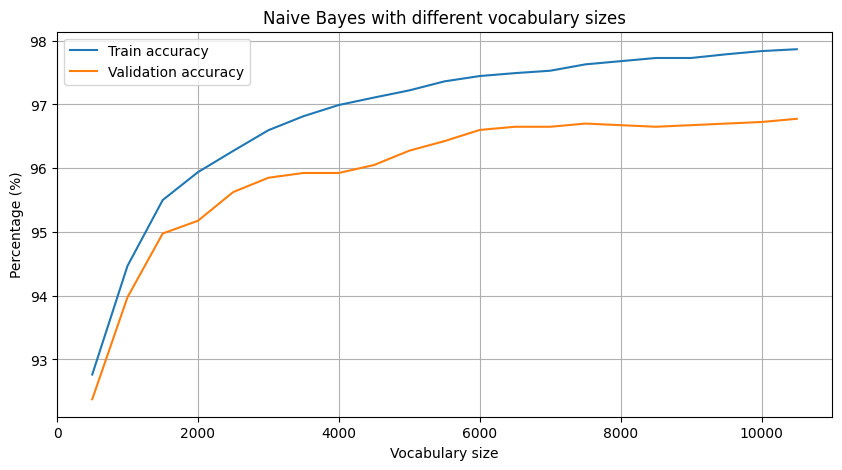
\includegraphics[width=\linewidth]{images/naive_voc_size.png}
    \end{subfigure}%
    \begin{subfigure}{.5\linewidth}
        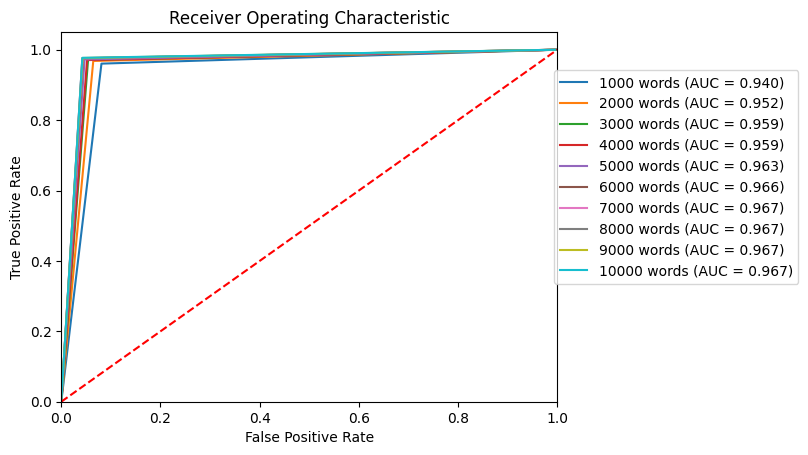
\includegraphics[width=\linewidth]{images/naive_voc_size_ROC.png}
    \end{subfigure}
    \caption{On left train and test accuracy, on right ROC and AUC for different vocabulary size}
    \label{fig-1}
\end{figure}
\subsubsection*{Features selection}
In the comparison of feature types, the performance in terms of validation accuracy and AUC was assessed for three different feature sets:
bag of words using the 6000 most frequent words, bag of words with the 6000 most frequent words excluding stop words,
and bag of words with the 6000 most frequent words utilizing stemming.\\
Figure 2 illustrates that the removal of stop words significantly reduces performance, both in accuracy and AUC.
This may be attributed to the fact that stop words, although semantically insignificant, play a crucial role in this particular classification task.\\
Conversely, stemming exhibits comparable performance to the classical bag of words approach.\\
As a result, the simplest option, the classical bag of words, emerges as the optimal choice, providing higher performance.

\begin{figure}[h]
    \begin{subfigure}{.5\linewidth}
        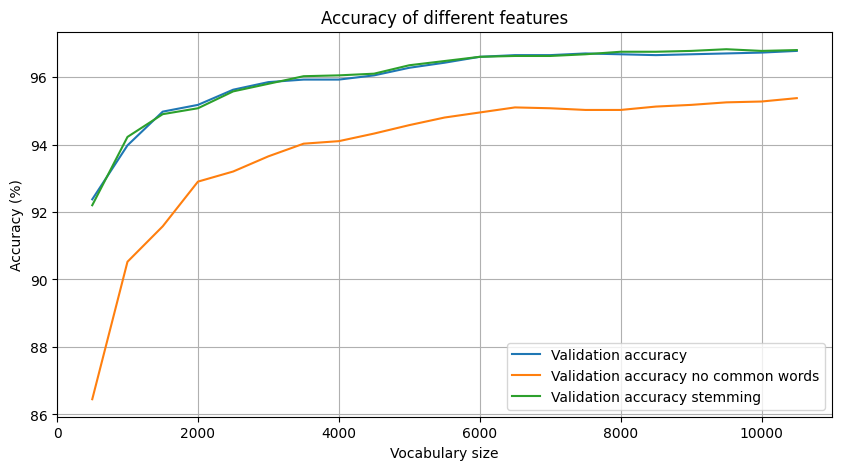
\includegraphics[width=\linewidth]{images/naive_features_sel.png}
    \end{subfigure}%
    \begin{subfigure}{.5\linewidth}
        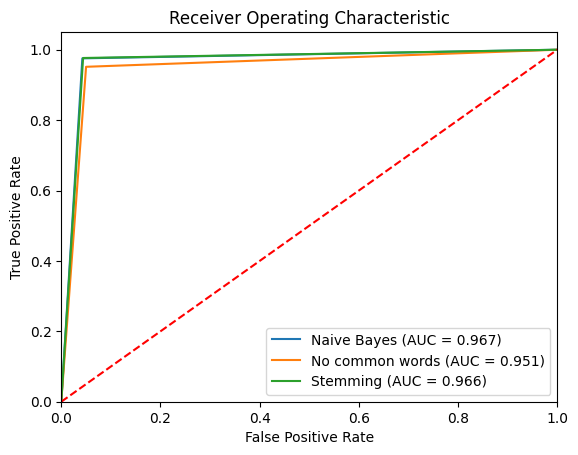
\includegraphics[width=\linewidth]{images/naive_features_sel_ROC.png}
    \end{subfigure}
    \caption{On left train and test accuracy, on right ROC and AUC for different features}
    \label{fig-2}
\end{figure}
\subsection{Analysis based on False Positive Rate}
\subsubsection*{size of the vocabulary}
As can be observed from the graph in Figure \ref{fig-3}, the false positive rate decreases as the size of the vocabulary increases,
reaching a relatively stable point beyond 7000 words.
This finding suggests that a vocabulary of 7000 words captures the most significant information without incurring overfitting.
\begin{figure}[h]
    \centering
    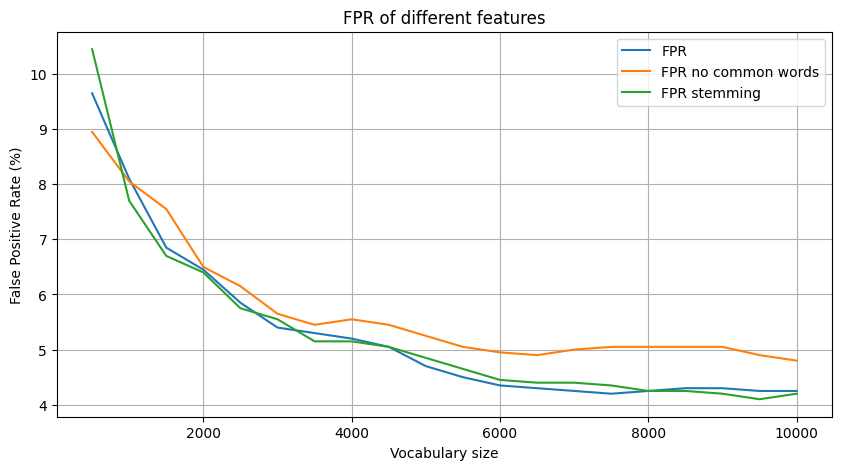
\includegraphics[width=0.7\columnwidth]{images/fpr_naive_voc_size_features_selection.png}
    \caption{False Positive Rate for different vocabulary size and for different features}
    \label{fig-3}
\end{figure}

\subsubsection*{Features selection}
Regarding the feature selection, as evident from the graph in Figure \ref{fig-3},
the utilization of stemming does not exhibit a significant impact on the false positive rate.
On the other hand, the removal of stop words negatively affects the false positive rate, causing it to be higher compared to the other features.
Therefore, the optimal choice is to utilize the bag of words approach with the top 7000 most frequent words,
without removing stop words and without employing stemming.

\subsubsection*{Choice of the bias}
If the aim is to further minimize the false positive rate, an adjustment to the bias can be made.
Altering the bias results in a change in the classification threshold, providing the ability to select a threshold that penalizes false positives more severely.
It is important, however, to exercise caution as reducing the false positive rate comes at the expense of a significant increase in the False Negative Rate,
thereby decreasing overall accuracy.
Consequently, the bias value must be chosen carefully to ensure that the trade-off between the two metrics is acceptable.\\
To assess the impact of different bias values on performance, various combinations within the range of $[-7, 7]$ were tested,
and both accuracy and false positive rate were calculated. Table \ref{tab-1} presents notable bias values along with their corresponding performance metrics.
The bias value of $[4, -5]$ was ultimately chosen since it exhibits an exceptionally low false positive rate while maintaining a reasonably high accuracy level.
\rowcolors{2}{green!8}{green!18}
\begin{table}[H]
    \centering
    \begin{tabular}{|c|c|c|}
        \hline
        Bias      & Accuracy (\%) & False Positive Rate (\%) \\
        \hline
        $[6, -4]$ & 84.950        & 0.05                     \\
        $[4, -5]$ & 87.525        & 0.10                     \\
        $[3, -5]$ & 89.750        & 0.25                     \\
        $[5, -2]$ & 91.650        & 0.35                     \\
        $[0, -6]$ & 93.275        & 0.45                     \\
        \hline
    \end{tabular}
    \caption{Accuracy and False Positive Rate for different bias}
    \label{tab-1}
\end{table}



\section{Logistic regression}
Logistic Regression is a widely used supervised machine learning algorithm for binary classification.
Unlike linear regression, which predicts continuous values, logistic regression models the probability of an instance belonging to a particular class.
It estimates the relationship between the input features and the log-odds of the target class using a logistic function.\\
In logistic regression, the model's parameters are learned by maximizing the likelihood function or minimizing the log loss
(also known as cross-entropy loss) during training.
The log loss measures the dissimilarity between the predicted probabilities and the actual class labels.
By minimizing the log loss, logistic regression aims to accurately classify instances and maximize the model's predictive performance.\\
Since there are a multitude of hyperparameters to tune, the adoption of a grid search approach was deemed impractical due to its high computational cost.
Consequently, a random search approach was employed instead to efficiently explore the hyperparameter space and identify the optimal configuration.
In this context, the tuning parameter $\lambda$ was specifically set to a value of $ 10^{-5}$.

\subsection{Analysis based on accuracy}
\subsubsection*{Learning rate}
To determine the optimal learning rate, a range of values spanning from $10^{-5}$ to $10^{-1}$ was systematically tested.
This investigation was carried out while utilizing a vocabulary size of 1000 words and performing 1000 iterations.\\
By analyzing the results, it becomes evident that the learning rate value of $3*10^{-3}$ emerges as the most favorable option,
as it maximizes the accuracy achieved on the validation set.
This conclusion is supported by the observations presented in Figure \ref{fig-4}.

\begin{figure}[h]
    \centering
    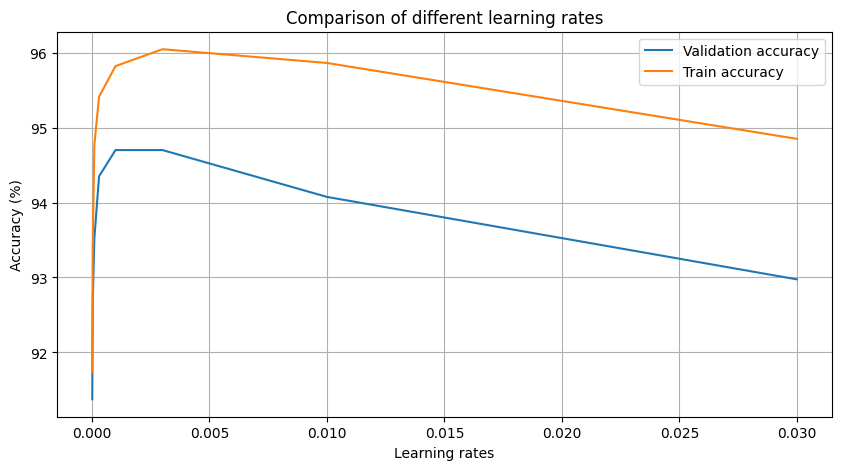
\includegraphics[width=0.7\columnwidth]{images/logreg_lr.png}
    \caption{Train and  validation accuracy for different learning rate}
    \label{fig-4}
\end{figure}

\subsubsection*{vocabulary size}


The impact of vocabulary size on the overall performance of the model was analyzed.
To conduct the analysis, a learning rate of $3 * 10^{-3}$ was used, and the model was trained for 1000 iterations.
The results, illustrated in Figure 5, provide valuable insights into the significant influence of vocabulary size on performance.
It was observed that the optimal vocabulary size for achieving the best performance is 8000 words.

\begin{figure}[h]
    \centering
    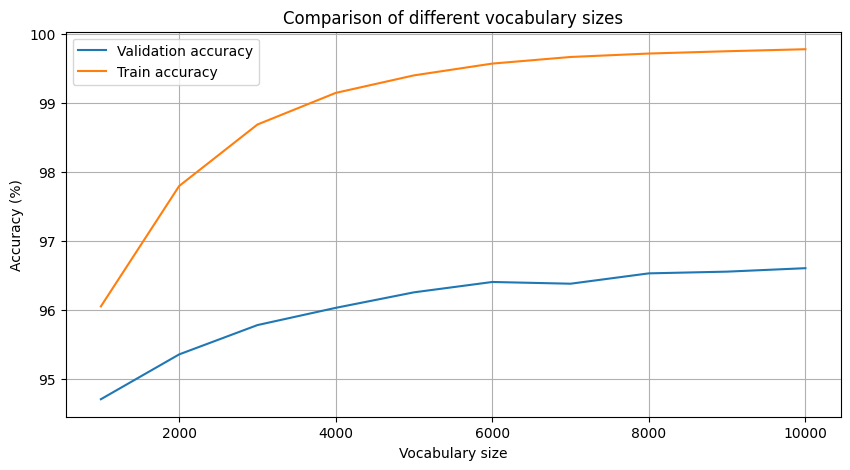
\includegraphics[width=0.7\columnwidth]{images/lr_voc_size.png}
    \caption{Train and  validation accuracy for different size of vocabulary}
    \label{fig-5}
\end{figure}


\subsubsection*{Features selection}
Regarding the feature selection, as evident from the graph in Figure \ref{fig-6}, it is observed that the model without
stop words has a lower AUC (Area Under the Curve) compared to the other two models.
On the other hand, the remaining two models exhibit the same area.
Based on this observation, the classic model was chosen as it does not require any further processing of the samples.
\begin{figure}[h]
    \centering
    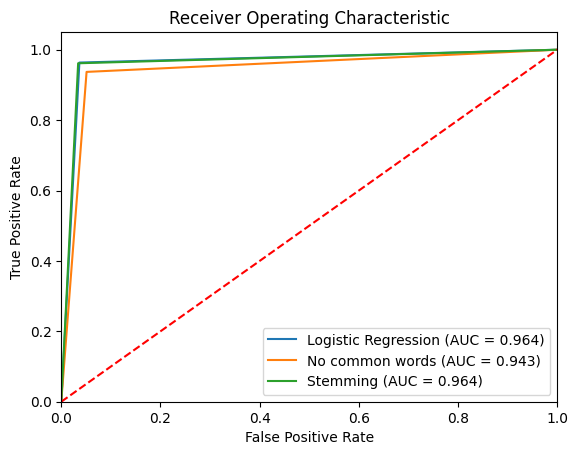
\includegraphics[width=0.7\columnwidth]{images/logreg_ROC_features_sel.png}
    \caption{ROC and AUC for different features}
    \label{fig-6}
\end{figure}


\subsubsection*{Number of iterations}
The impact of the number of iterations on the model's performance was thoroughly examined.
The obtained results, as depicted in Figure \ref{fig-7}, unequivocally demonstrate a direct relationship between the number of iterations and
the accuracy of the model. Notably, as the number of iterations increases, the accuracy of the model consistently improves.
This positive correlation holds true up to approximately 600 iterations, beyond which a slight decrease in accuracy is observed.

\begin{figure}[h]
    \centering
    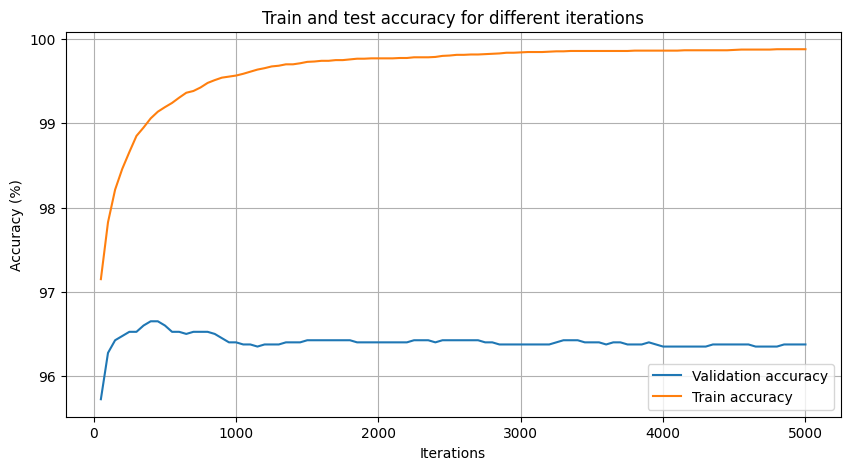
\includegraphics[width=0.7\columnwidth]{images/logreg_iter.png}
    \caption{Train and validation accuracy for different number of iterations}
    \label{fig-7}
\end{figure}

\subsection{Analysis based on False Positive Rate}
\subsubsection*{Learning rate}

Once again, a range of learning rates, spanning from $10^{-5}$ to $10^{-1}$, was explored.
The results, depicted in Figure \ref{fig-8}, clearly demonstrate that as the learning rate increases, the false positive rate (FPR) consistently decreases.
This downward trend continues until a learning rate of $10^{-2}$, beyond which the FPR stabilizes.
Considering the objective of minimizing the risk of skipping the loss function's minimum point, a learning
rate of $10^{-2}$ was ultimately selected as the optimal choice.
\begin{figure}[h]
    \centering
    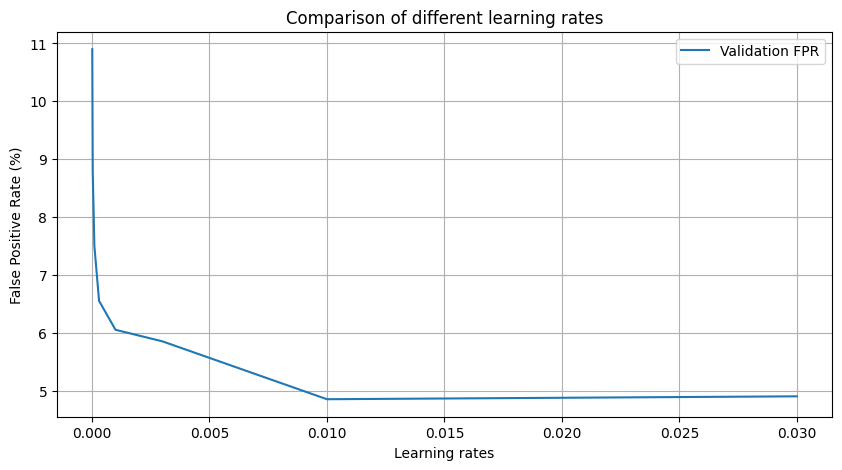
\includegraphics[width=0.7\columnwidth]{images/fpr_logreg_lr.png}
    \caption{False Positive Rate for different values of the learning rate}
    \label{fig-8}
\end{figure}
\subsubsection*{Size of the vocabulary}
As shown in figure \ref{fig-9}, the false positive rate decreases as the size of the vocabulary increases,
reaching a relatively stable point beyond 8000 words, with a value of 3.3\%.
\begin{figure}[h]
    \centering
    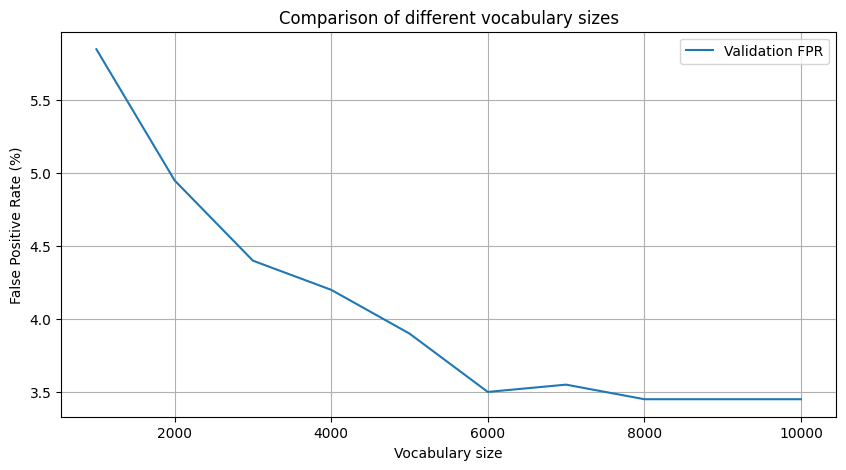
\includegraphics[width=0.7\columnwidth]{images/fpr_logreg_voc_size.png}
    \caption{FPR for different size of vocabulary}
    \label{fig-9}
\end{figure}
\subsubsection*{Features selection}
As we can see from the table below, the model that uses the classic bag of words and the BOW with stemming have the same FPR.
While the model that removes stop words has the highest false positive rate.
So the selected model is the one that uses the classic bag of words.
\rowcolors{2}{green!8}{green!18}
\begin{table}[H]
    \centering
    \begin{tabular}{|c|c|}
        \hline
        Feature                    & FPR (\%) \\
        \hline
        BOW without stopping words & 5.05     \\
        BOW with stemming          & 3.40     \\
        BOW                        & 3.40     \\
        \hline
    \end{tabular}
    \caption{FPR for different features}
    \label{tab-2}
\end{table}

\subsubsection*{Number of iterations}
As shown in the graph in Figure \ref{fig-10}, the false positive rate decreases as the number of iterations increases,
reaching a relatively stable point beyond 800 iterations, with a value of 3.35\%.

\begin{figure}[h]
    \centering
    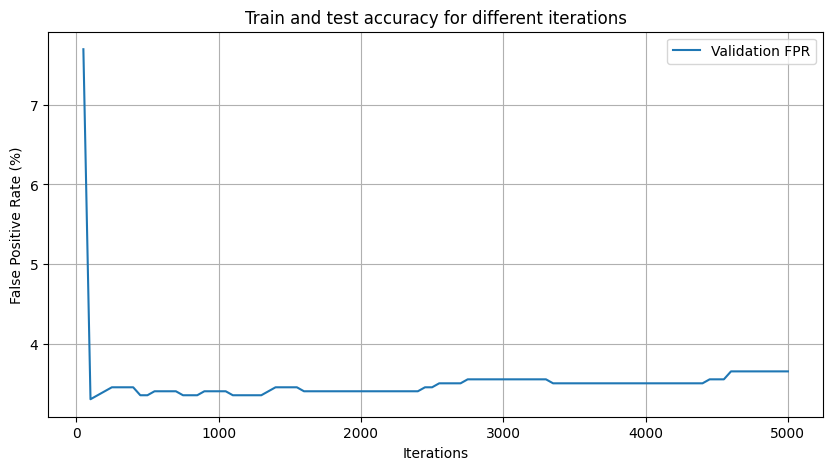
\includegraphics[width=0.7\columnwidth]{images/fpr_logreg_iters.png}
    \caption{FPR for different iterations}
    \label{fig-10}
\end{figure}
\subsubsection*{Choice of the bias}
As in the Na\"ive Bayes model, the bias can be adjusted to further minimize the false positive rate.
The bias value was varied within the range of $[-10, 10]$, and the corresponding accuracy and false positive rate were calculated.
Table \ref{tab-3} presents notable bias values along with their corresponding performance metrics.
The bias value of $-5$ was ultimately chosen since it exhibits an exceptionally low false positive rate while maintaining a reasonably high accuracy level,
which is also higher than the one obtained with the Na\"ive Bayes model.

\rowcolors{2}{green!8}{green!18}
\begin{table}[H]
    \centering
    \begin{tabular}{|c|c|c|}
        \hline
        Bias & Accuracy (\%) & False Positive Rate (\%) \\
        \hline
        -5   & 86.80         & 0.05                     \\
        -4   & 90.20         & 0.15                     \\
        -3   & 93.15         & 0.35                     \\
        \hline
    \end{tabular}
    \caption{Accuracy and False Positive Rate for different bias}
    \label{tab-3}
\end{table}
\section{Analysis of the best model}

\subsection{Analysis based on accuracy}
When evaluating the top-performing models for each algorithm, an analysis of the results reveals noteworthy insights.
The Naïve Bayes classifier exhibits an impressive accuracy of 96.675\%, while Logistic Regression follows closely with an accuracy of 96.45\%.
Additionally, as depicted in Figure \ref{fig-11}, the Naïve Bayes model showcases a slightly larger area under the curve compared to Logistic Regression.
This indicates that Naïve Bayes outperforms Logistic Regression in terms of overall predictive capability.
Furthermore, it is worth noting that Naïve Bayes offers the added advantage of being easier to implement and train.
Taking all factors into consideration, Naïve Bayes emerges as the preferred model for this task.

\begin{figure}[h]
    \centering
    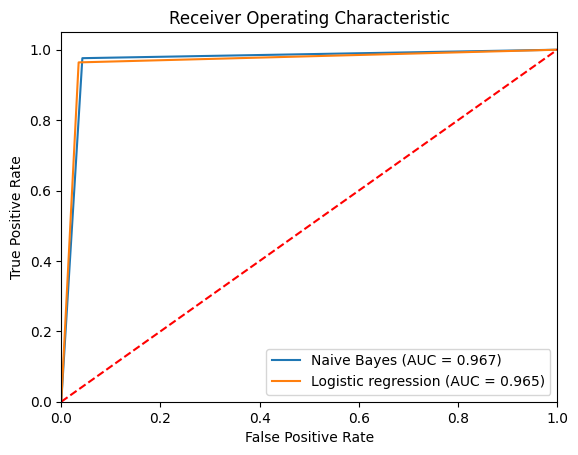
\includegraphics[width=0.6\columnwidth]{images/comparison.png}
    \caption{ROC and AUC for the two models}
    \label{fig-11}
\end{figure}

\subsubsection*{Confusion matrix}
The confusion matrix is a important tool in evaluating the performance of a binary classification model.
It presents a comprehensive view of the model's predictions, displaying the count of correct and incorrect predictions for each class.\\
Figure \ref{fig-12} showcases the confusion matrix obtained from the Na\"ive Bayes model.
The depicted confusion matrix underscores the exceptional performance of the model.
It exhibits a substantial number of accurate predictions while demonstrating a minimal count of erroneous predictions.
Such results strongly indicate the model's effectiveness in correctly classifying instances and highlight its proficiency
in distinguishing between the two classes.
\begin{figure}[h]
    \centering
    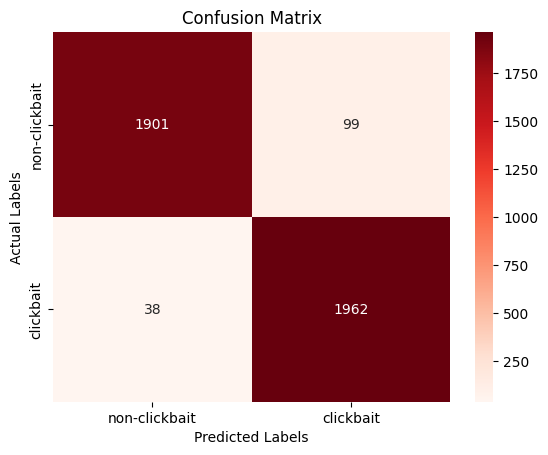
\includegraphics[width=0.5\columnwidth]{images/naive_conf_matrix.png}
    \caption{Confusion matrix for the Na\"ive Bayes model}
    \label{fig-12}
\end{figure}
\subsubsection*{Most impactful words}

To delve deeper into the model's performance, the most significant words for classification were identified,
focusing on those with a substantial difference in weight between the two classes.
Specifically, they selected the top 10 words with the largest magnitude difference across both classes.
The results of this analysis are visually presented in Figure \ref{fig-13},
providing valuable information about the discriminative power of these influential words.
\begin{figure}[h]
    \begin{subfigure}{.5\linewidth}
        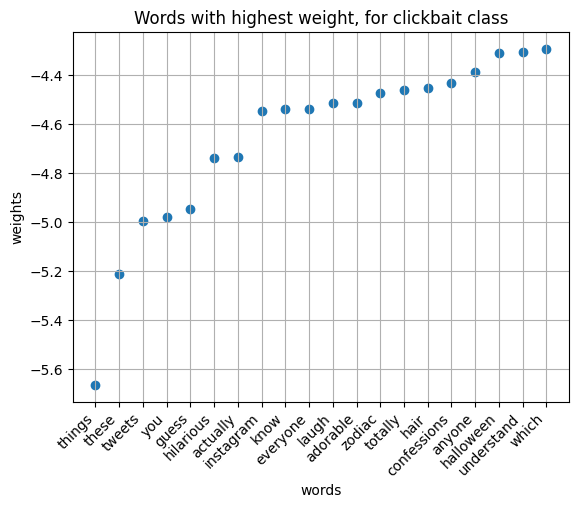
\includegraphics[width=\linewidth]{images/naive_click_weights.png}
    \end{subfigure}%
    \begin{subfigure}{.5\linewidth}
        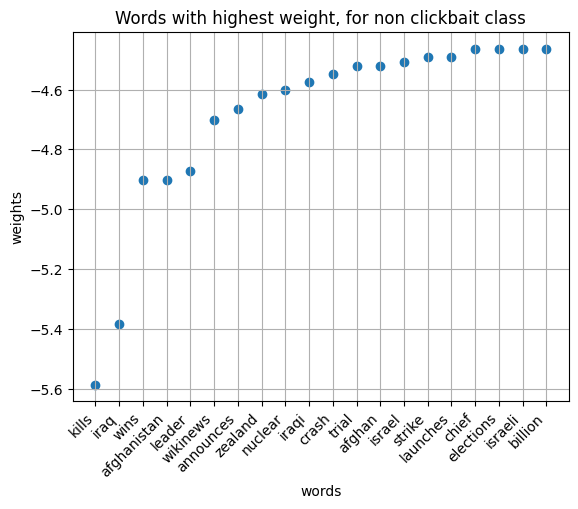
\includegraphics[width=\linewidth]{images/naive_no_click_weights.png}
    \end{subfigure}
    \caption{Most impactful words for classification. On left for clickbait, on right for non-clickbait}
    \label{fig-13}
\end{figure}

\subsection{Analysis based on False Positive Rate}
Considering the results presented in Tables \ref{tab-1} and \ref{tab-3}, the comparison reveals that
the model utilizing Logistic Regression exhibits a marginally higher accuracy while maintaining the same False Positive Rate (FPR).
However, it is important to note that Logistic Regression involves the optimization of numerous hyperparameters and requires a longer training time.
Consequently, selecting the optimal model is not a straightforward decision. If the primary objective is to obtain the highest performing model,
then Logistic Regression proves to be the preferred choice.
On the other hand, if simplicity and faster training are prioritized,
Na\"ive Bayes emerges as the more suitable option. In this particular scenario, the Na\"ive Bayes model was selected due to its simplicity and efficiency
in the training process.
\subsubsection*{Confusion matrix}
In Figure \ref{fig-14}, the confusion matrix derived from the Naïve Bayes model is presented.
The analysis reveals a notable reduction in the false positive rate compared to the previous model.
One instance in 2000 were falsely identified as clickbait, despite being non-clickbait content.
However, it is worth noting that this improvement came at the cost of an increase in false negatives,
which rose from 38 to 471 misclassified instances.
\begin{figure}[h]
    \centering
    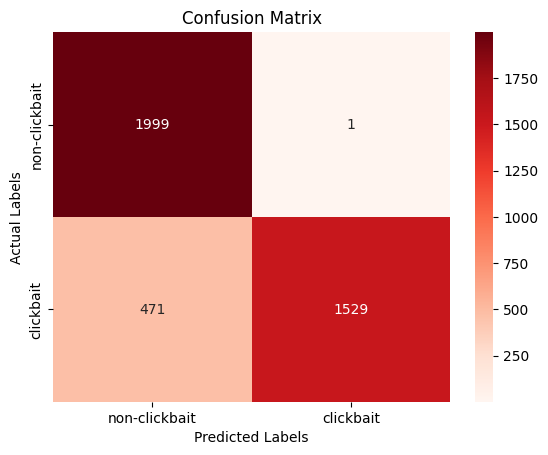
\includegraphics[width=0.5\columnwidth]{images/fpr_naive_conf_matrix.png}
    \caption{Confusion matrix for the Na\"ive Bayes model}
    \label{fig-14}
\end{figure}

\section{Declaration}
I affirm that this report is the result of my own work and that I did not share any part of it with anyone
else except the teacher.
\end{document}